\documentclass{beamer}

% For more theme options:
%/usr/share/texmf/tex/latex/beamer/base/themes/theme/compatibility
\usepackage{beamerthemelined}

% this package seems to throw an error for me. -Juneki 12/6/14
%\usepackage[usenames,dvipsnames,svgnames,table]{xcolor}
\usepackage{soul}

\usepackage{algorithm}
\usepackage[noend]{algpseudocode}
\usepackage{graphicx}
\usepackage{caption}
\usepackage{subcaption}

\usepackage{tikz-dependency}

\newcommand{\eqnref}[1]{\eqref{eqn:#1}}
%\usepackage[usenames,dvipsnames,svgnames,table]{xcolor}  % allows better color names
\usepackage{todonotes}   % insert [disable] to disable all notes
\newcommand{\Note}[4][]{\todo[author=#2,color=#3,fancyline,#1]{#4}}
\newcommand{\noteJH}[2][]{\Note[#1]{JH}{blue!40}{#2}}
\newcommand{\noteJE}[2][]{\Note[#1]{JE}{green!40}{#2}}
\newcommand{\notewho}[3][]{\Note[#1]{#2}{orange!40}{#3}}  % extra arg with miscellaneous author
\newcommand{\NoteJH}[2][]{\noteJH[inline,#1]{#2}}
\newcommand{\NoteJE}[2][]{\noteJE[inline,#1]{#2}}
\newcommand{\Notewho}[3][]{\notewho[inline,#1]{#2}{#3}}  % extra arg with miscellaneous author



\begin{document}
\title{Deriving Multi-Headed Planar Dependency Parses from Link Grammar Parses}
\author{Juneki Hong, Jason Eisner}
\date{\today}
\frame{\titlepage}

\section{Motivation}
\frame{\frametitle{Motivation}
  \begin{itemize}
    \item We need a multiheaded dependency corpus for parsing
  \end{itemize}
}

\section{Multi-headed}

\frame{\frametitle{Multi-headedness}
  \begin{itemize}
    \item Control
    \item Relativization
    \item Conjunction
  \end{itemize}
}

\subsection{Control}
\frame{\frametitle{Control}
  \begin{figure}
    \begin{dependency}
      \begin{deptext}
        Jill \& likes \& to \& skip \\
      \end{deptext}
      \depedge[edge above, thick, hide label]{2}{1}{}
      \depedge[edge below, ultra thick, hide label, edge style = {purple}, edge unit distance = 1.5ex]{4}{1}{}
      \depedge[edge above, thick, hide label]{2}{3}{}
      \depedge[edge above, thick, hide label]{3}{4}{}
    \end{dependency}
    \caption*{Jill is the subject of two verbs}
  \end{figure}

  \begin{figure}
    \begin{dependency}
      \begin{deptext}
        Jill \& persuaded \& Jack \& to \& skip \\
      \end{deptext}
      \depedge[edge above, thick, hide label]{2}{1}{}
      \depedge[edge above, thick, hide label]{2}{3}{}
      \depedge[edge above, thick, hide label]{3}{4}{}
      \depedge[edge above, thick, hide label]{4}{5}{}
      \depedge[edge below, ultra thick, hide label, edge style = {purple}, edge unit distance = 1.5ex]{3}{5}{}
    \end{dependency}
    \caption*{Jack is the object of one verb and the subject of another}
  \end{figure}
}


\subsection{Relativization}
\frame{\frametitle{Relativization}
  \begin{figure}
    \begin{dependency}
      \begin{deptext}
        The \& boy \& that \& Jill \& skipped \& with \& fell \& down \\
      \end{deptext}
      \depedge[edge above, thick, hide label]{2}{1}{}
      \depedge[edge above, thick, hide label]{2}{3}{}
      \depedge[edge above, thick, hide label]{3}{4}{}
      \depedge[edge above, thick, hide label]{4}{5}{}
      \depedge[edge above, thick, hide label]{5}{6}{}
      \depedge[edge above, thick, hide label]{2}{7}{}
      \depedge[edge above, thick, hide label]{7}{8}{}
      \depedge[edge below, ultra thick, hide label, edge style = {purple}, edge unit distance = 1.5ex]{6}{2}{}
    \end{dependency}
    \caption*{The boy is the object of ``with'' as well as the subject of ``fell''.}
  \end{figure}
}


\subsection{Conjunction}
\frame{\frametitle{Conjunction}
  \begin{figure}
    \begin{dependency}
      \begin{deptext}
        Jack \& and \& Jill \& went \& up \& the \& hill \\
      \end{deptext}
      \depedge[edge above, thick, hide label]{2}{1}{}
      \depedge[edge above, thick, hide label]{2}{3}{}
      \depedge[edge above, thick, hide label]{4}{2}{}
      \depedge[edge above, thick, hide label]{4}{5}{}
      \depedge[edge above, thick, hide label]{5}{7}{}
      \depedge[edge above, thick, hide label]{7}{6}{}

      \depedge[edge below, ultra thick, hide label, edge style = {purple}, edge unit distance = 1.5ex]{4}{1}{}
      \depedge[edge below, ultra thick, hide label, edge style = {purple}, edge unit distance = 1.5ex]{4}{3}{}

    \end{dependency}
    \caption*{Jack and Jill serve as the two arguments to and, but they are also semantically subjects of went.}
  \end{figure}
}



%\frame{\frametitle{Multi-headedness}
%  \begin{figure}
%    \begin{dependency}
%      \begin{deptext}
%      I \& think \& the \& man \& who \& you \& saw \& wants \& to \& eat \& sushi \\
%      \end{deptext}
%      \deproot[edge above, thick]{2}{ROOT}
%      \depedge[edge above, thick, hide label]{2}{1}{} % think -> I
%      \depedge[edge above, thick, hide label]{4}{3}{} % man -> the
%      \depedge[edge above, thick, hide label]{4}{5}{} % man -> who
%      \depedge[edge above, thick, hide label]{7}{6}{} % saw -> you
%      \depedge[edge above, thick, hide label]{8}{4}{} % wants -> man
%      \depedge[edge above, thick, hide label]{4}{7}{} % man -> saw
%      \depedge[edge above, thick, hide label]{2}{8}{} % think -> wants
%      \depedge[edge above, thick, hide label]{8}{10}{} % wants -> eat
%      \depedge[edge above, thick, hide label]{10}{9}{} % eat -> to
%      \depedge[edge above, thick, hide label]{10}{11}{} % eat -> sushi
%      \depedge[edge below, edge style = {purple}, hide label, edge unit distance = 1.5ex, ultra thick]{10}{4}{} % eat -> man
%    \end{dependency}
%    \caption*{Example of a Multiheaded Parse}
%  \end{figure}
%}



% Shouldn't mention non-projectivity. 
%\frame{\frametitle{Non-projectivity}
%\begin{figure}
%  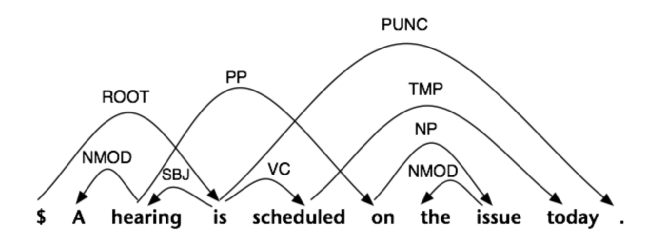
\includegraphics[width=\linewidth]{multiheaded}
%  \caption*{English is not a completely projective language}
%  \NoteJH{image taken from Chris Dyer's slide: http://demo.clab.cs.cmu.edu/fa2014-11711/images/0/0e/Depparsing.pdf}
%  \NoteJH{I should also ask Chris for permission to use this}
%\end{figure}
%}


\section{Non Projectivity}
\frame{\frametitle{We do not address: Non-Projectivity}
\begin{itemize}
  \item Projectivity assumptions allow us to have efficient parsing algorithms that utilize dynamic programming
  \item English is mostly projective
\end{itemize}
}

\frame{\frametitle{We do not address: Non-Projectivity}
\begin{itemize}
  \item Projectivity assumptions allow us to have efficient parsing algorithms that utilize dynamic programming
  \item English is mostly projective
\end{itemize}

\begin{figure}
  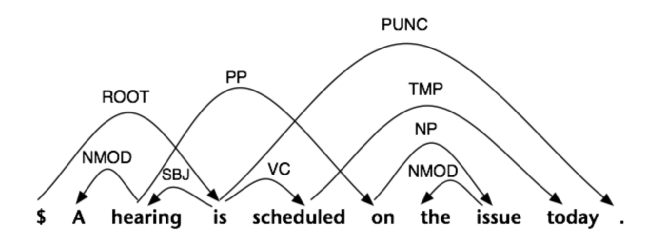
\includegraphics[width=0.7\linewidth]{multiheaded}
  \caption*{But not always}
  \NoteJH{image taken from Chris Dyer's slide: http://demo.clab.cs.cmu.edu/fa2014-11711/images/0/0e/Depparsing.pdf}
  \NoteJH{I should also ask Chris for permission to use this}
\end{figure}


}


\section{Link Grammars}

\frame{\frametitle{Link Grammars}
  \begin{enumerate}
    \item Grammar-based formalism for projective dependency parsing with undirected links
  \end{enumerate}
}


\frame{\frametitle{Link Grammars}
\begin{figure}
  \begin{dependency}[edge style={-}]
	\begin{deptext}
	  the \& matter \& may \& never \& even \& be \& tried \& in \& court \& . \\
	  - \& n-u \& v \& e \& e \& v \& v-d \& r \& n-u \& - \\
	\end{deptext}
	\depedge[edge above, thick, edge style = {red}]{2}{3}{S}
	\depedge[edge above, thick, edge style = {red}]{3}{6}{I}
	\depedge[edge above, thick, edge style = {red}]{2}{1}{D}
	\depedge[edge above, thick, edge style = {red}]{7}{8}{MV}
	\depedge[edge above, thick, edge style = {red}]{6}{7}{P}
	\depedge[edge above, thick, edge style = {red}]{8}{9}{J}
	\deproot[edge above, thick, edge style = {red}]{2}{W}
	\deproot[edge above, thick, edge style = {red}]{7}{WV}
	\deproot[edge above, thick, edge style = {red}]{10}{X}
	\depedge[edge above, thick, edge style = {red}]{6}{4}{E}
	\depedge[edge above, thick, edge style = {red}]{6}{5}{E}
  \end{dependency}
  \caption*{Link Parse of a sentence from Penn Tree Bank}
\end{figure}


}

\frame{\frametitle{Link Grammars}
\begin{figure}
  \begin{dependency}
	\begin{deptext}
	  the \& matter \& may \& never \& even \& be \& tried \& in \& court \& . \\
	  - \& n-u \& v \& e \& e \& v \& v-d \& r \& n-u \& - \\
	\end{deptext}
	\depedge[edge above, thick, edge style = {red}]{2}{3}{S}
	\depedge[edge above, thick, edge style = {red}]{3}{6}{I}
	\depedge[edge above, thick, edge style = {red}]{2}{1}{D}
	\depedge[edge above, thick, edge style = {red}]{7}{8}{MV}
	\depedge[edge above, thick, edge style = {red}]{6}{7}{P}
	\depedge[edge above, thick, edge style = {red}]{8}{9}{J}
	\deproot[edge above, thick, edge style = {red}]{2}{W}
	\deproot[edge above, thick, edge style = {red}]{7}{WV}
	\deproot[edge above, thick, edge style = {red}]{10}{X}
	\depedge[edge above, thick, edge style = {red}]{6}{4}{E}
	\depedge[edge above, thick, edge style = {red}]{6}{5}{E}
  \end{dependency}

  \caption*{Directionalize the edges}
\end{figure}
}


\frame{\frametitle{Link Grammars}
\begin{figure}
  \begin{dependency}
	\begin{deptext}
	  {\scriptsize DT} \& {\scriptsize NN} \& {\scriptsize MD} \& {\scriptsize RB} \& {\scriptsize RB} \& {\scriptsize VB} \& {\scriptsize VB} \& {\scriptsize IN} \& {\scriptsize NN} \& {\scriptsize .} \\
	  the \& matter \& may \& never \& even \& be \& tried \& in \& court \& . \\
	  - \& n-u \& v \& e \& e \& v \& v-d \& r \& n-u \& - \\
	\end{deptext}
	\deproot[edge above, thick, edge style = {blue}]{3}{\small ROOT}
	\depedge[edge below, thick, edge style = {red}]{2}{3}{S}
	\depedge[edge above, thick, edge style = {blue}]{3}{2}{\small SBJ}
	\depedge[edge above, thick, edge style = {blue}]{3}{4}{\small ADV}
	\depedge[edge above, thick, edge style = {blue}]{3}{5}{\small ADV}
	\depedge[edge below, thick, edge style = {red}]{3}{6}{I}
	\depedge[edge above, thick, edge style = {blue}]{3}{6}{\small VC}
	\depedge[edge above, thick, edge style = {blue}, edge unit distance =1.5ex]{3}{10}{\small P}
	\depedge[edge below, thick, edge style = {red}]{2}{1}{D}
	\depedge[edge above, thick, edge style = {blue}]{2}{1}{\small NMOD}
	\depedge[edge below, thick, edge style = {red}]{7}{8}{MV}
	\depedge[edge above, thick, edge style = {blue}]{7}{8}{\small ADV}
	\depedge[edge below, thick, edge style = {red}]{6}{7}{P}
	\depedge[edge above, thick, edge style = {blue}]{6}{7}{\small VC}
	\depedge[edge below, thick, edge style = {red}]{8}{9}{J}
	\depedge[edge above, thick, edge style = {blue}]{8}{9}{\small PMOD}
	\deproot[edge below, thick, edge style = {red}]{2}{W}
	\deproot[edge below, thick, edge style = {red}]{7}{WV}
	\deproot[edge below, thick, edge style = {red}]{10}{X}
	\depedge[edge below, thick, edge style = {red}]{6}{4}{E}
	\depedge[edge below, thick, edge style = {red}]{6}{5}{E}
  \end{dependency}

  \caption*{Compare resulting dependency parse with Penn Treebank annotations}
\end{figure}


}



\frame{\frametitle{Link Grammars}
\begin{figure}
  \begin{dependency}
	\begin{deptext}
	  {\scriptsize DT} \& {\scriptsize NN} \& {\scriptsize MD} \& {\scriptsize RB} \& {\scriptsize RB} \& {\scriptsize VB} \& {\scriptsize VB} \& {\scriptsize IN} \& {\scriptsize NN} \& {\scriptsize .} \\
	  the \& matter \& may \& never \& even \& be \& tried \& in \& court \& . \\
	  - \& n-u \& v \& e \& e \& v \& v-d \& r \& n-u \& - \\
	\end{deptext}
	\deproot[edge above, edge style = {blue, dotted}]{3}{\small ROOT}
	\depedge[edge below, edge style = {red, ultra thick}]{2}{3}{S}
	\depedge[edge above, edge style = {blue, ultra thick}]{3}{2}{\small SBJ}
	\depedge[edge above, edge style = {blue, dotted}]{3}{4}{\small ADV}
	\depedge[edge above, edge style = {blue, dotted}]{3}{5}{\small ADV}
	\depedge[edge below, edge style = {red, thick}]{3}{6}{I}
	\depedge[edge above, edge style = {blue, thick}]{3}{6}{\small VC}
	\depedge[edge above, edge style = {blue, dotted}, edge unit distance =1.5ex]{3}{10}{\small P}
	\depedge[edge below, edge style = {red, thick}]{2}{1}{D}
	\depedge[edge above, edge style = {blue, thick}]{2}{1}{\small NMOD}
	\depedge[edge below, edge style = {red, thick}]{7}{8}{MV}
	\depedge[edge above, edge style = {blue, thick}]{7}{8}{\small ADV}
	\depedge[edge below, edge style = {orange, thick}]{6}{7}{P}
	\depedge[edge above, edge style = {blue, thick}]{6}{7}{\small VC}
	\depedge[edge below, edge style = {red, thick}]{8}{9}{J}
	\depedge[edge above, edge style = {blue, thick}]{8}{9}{\small PMOD}
	\deproot[edge below, edge style = {red, dotted}]{2}{W}
	\deproot[edge below, edge style = {orange, ultra thick, dotted}]{7}{WV}
	\deproot[edge below, edge style = {red, dotted}]{10}{X}
	\depedge[edge below, edge style = {red, dotted}]{6}{4}{E}
	\depedge[edge below, edge style = {red, dotted}]{6}{5}{E}
  \end{dependency}

  \caption*{Compare resulting dependency parse with Penn Treebank annotations}
\end{figure}


}


\section{ILP}
\frame{\frametitle{Integer Linear Programming}

\NoteJH{Will the audience know about ILP?}


}


\section{ILP Model}
\frame{\frametitle{Integer Linear Programming Model}

\NoteJH{Take from the paper.}

}



\section{Experiments and Results}
\frame{\frametitle{Experiments and Results}

}



\section{Conclusions}
\frame{\frametitle{Conclusions}

}


%\nocite{*}
%\bibliographystyle{plain}
%\bibliography{hong+eisner.TLT13.slides.bib}
%\appendix

\end{document}
